% !TEX root = ../sethomas_thesis_main.tex

\chapter{Predicting the Shape Memory Effect}\label{chap:sma-model}
\section{Introduction}
% Intro to thermal SMAs (mention magnetic)
% Type of TSMA (NiTi, CuAl)
    % Mechanical prop of NiTi (table)
% SME and SE
% SME graph A to M, detw to tw
% Phase transformations
\begin{figure}[hbt]
    \centering
    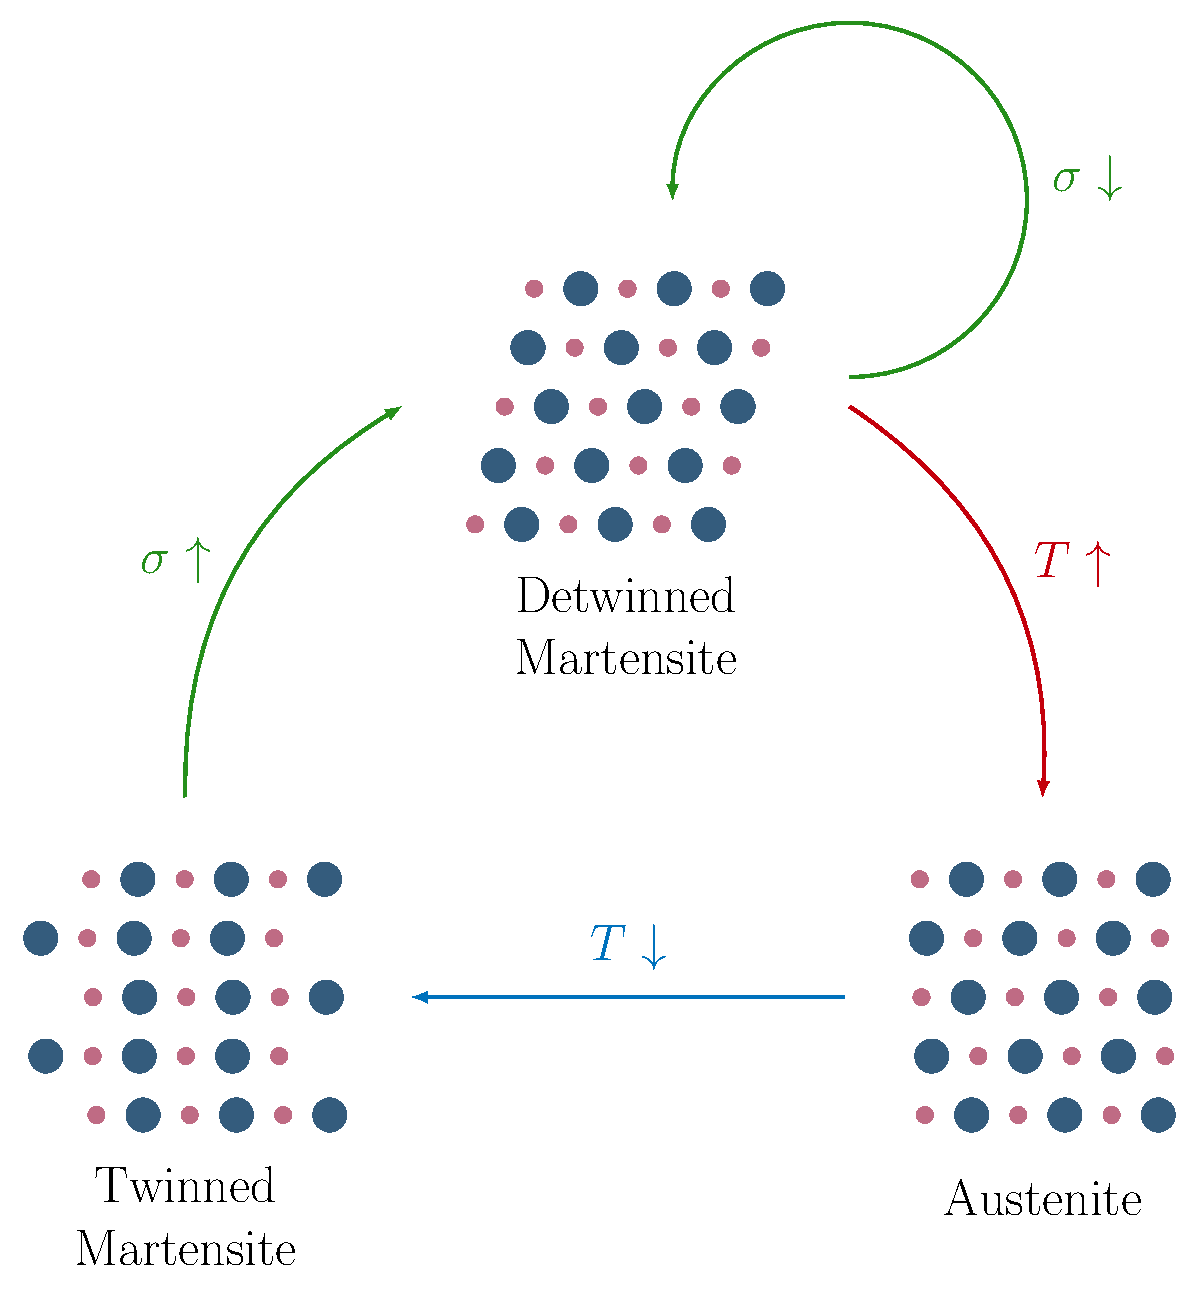
\includegraphics[width=0.6\textwidth]{images/chap2/sma-phases.pdf}
    \caption{A schematic representation of the Shape Memory Effect (SME) showing the different phase transformations and crystal structures.}
    \label{fig:sma-phases}
\end{figure}

\begin{figure}[hbt]
    \centering
    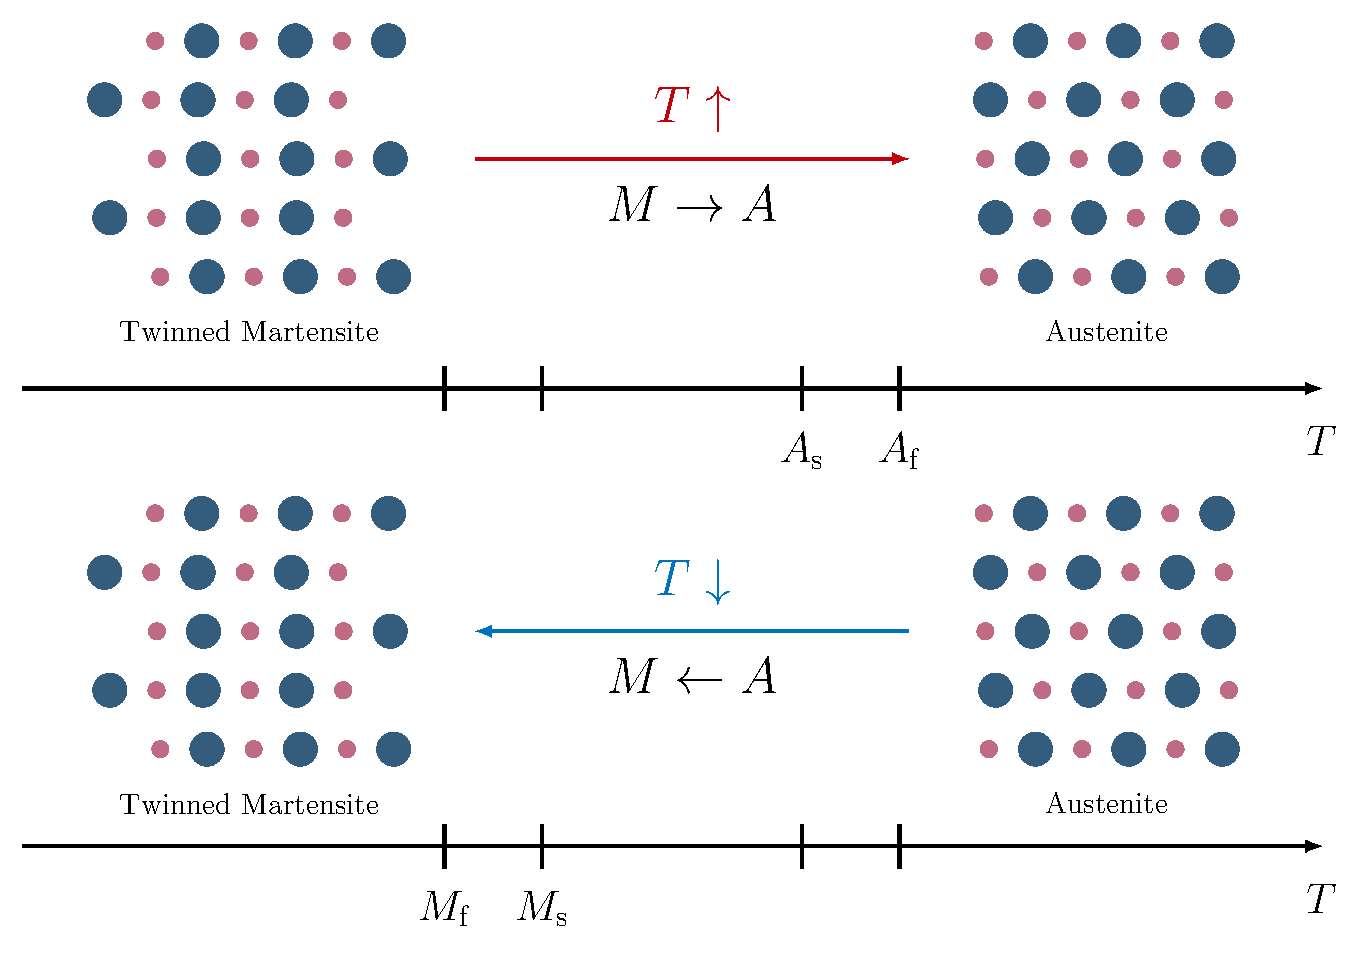
\includegraphics[width=0.9\textwidth]{images/chap2/sma-phase-transformations.pdf}
    \caption{A visual representation of the phase transformations that occur during Shape Memory Effect (SME).}
    \label{fig:sma-phase-transformations}
\end{figure}
\section{Analytical Modelling of the SME}
% Phenomenological modelling
% DSC
% Types and history of models
% Brinson model
% Temp vs Martensite %
% SME graph
\section{Finite Element Modelling}
\section{Stroke Estimation of SMA Actuators}
\subsection{Mechanical Modelling}
\subsection{Thermal Model}
\section{Simplified SMA Actuator Model}\label{sec:simplified-sma-model}
\section{Summary and Conclusion}
In this chapter, different modelling strategies, such as finite element modelling and analytical modelling, are presented. Here, the modelling techniques are employed in the context of the traditional SMA actuator design methodology. Furthermore, the bias spring actuator model and a simplified model are presented.
